
\chapter{Funktionen}
\section{Elementare Funktionen}
\subsection{Exponentialfunktion}
\begin{definition}[Exponentialfunktion]\mbox{}\newline
Für $x\in\C$ als $\C\to\C$:
\begin{equation}
\exp(x) := \sum_{k=0}^{\infty} \frac{x^k}{k!}
= 1+x+\frac{x^2}{2}+\frac{x^3}{6}+\ldots
\end{equation}
\end{definition}

\noindent
\strong{Eigenschaften.}
Die Einschränkung von $\exp$ auf $\R$ ist injektiv und
besitzt die Bildmenge $\R^+$.

Die Exponentialfunktion ist holomorph auf ganz $\C$ und stimmt
mit ihrer eigenen Ableitung überein:
\begin{equation}
\exp'(x) = \exp(x).
\end{equation}
Für $x,y\in\C$ gilt:
\begin{gather}
\exp(x+y) = \exp(x)\exp(y),\\
\exp(x-y) = \frac{\exp(x)}{\exp(y)},\\
\exp(-x) = \frac{1}{\exp(x)}.
\end{gather}
\strong{Eulersche Formel.} Für $x\in\C$ gilt:
\begin{equation}
\ee^{\ui x} = \cos x+\ui\sin x.
\end{equation}

\subsection{Logarithmusfunktion}
\begin{definition}[Natürlicher Logarithmus]\mbox{}\newline
Für $x\in\R^+$ als $\R^+\to\R$:
\begin{equation}
\ln(x) := \exp^{-1}(x).
\end{equation}
Für $z\in\C\setminus\{0\}$, $z=r\ee^{\ui\varphi}$ als
$\C\setminus\{0\}\to\C$:
\begin{equation}
\ln(z):=\ln(r)+\ui\varphi.
\end{equation}
\end{definition}
\noindent
\strong{Eigenschaften.}
Für $x\in\R^+$ gilt:
\begin{equation}
\ln(x):=\int_1^x \frac{1}{t}\,\mathrm dt.
\end{equation}

Für $z\in\C\setminus\{0\}$ gilt:
\begin{equation}
\ln(z)=\lim_{h\to 0}\frac{z^h-1}{h}.
\end{equation}
Die Logarithmusfunktion ist auf $\C{\setminus}\R_0^-$ holomorph.

%\begin{figure}[h]
%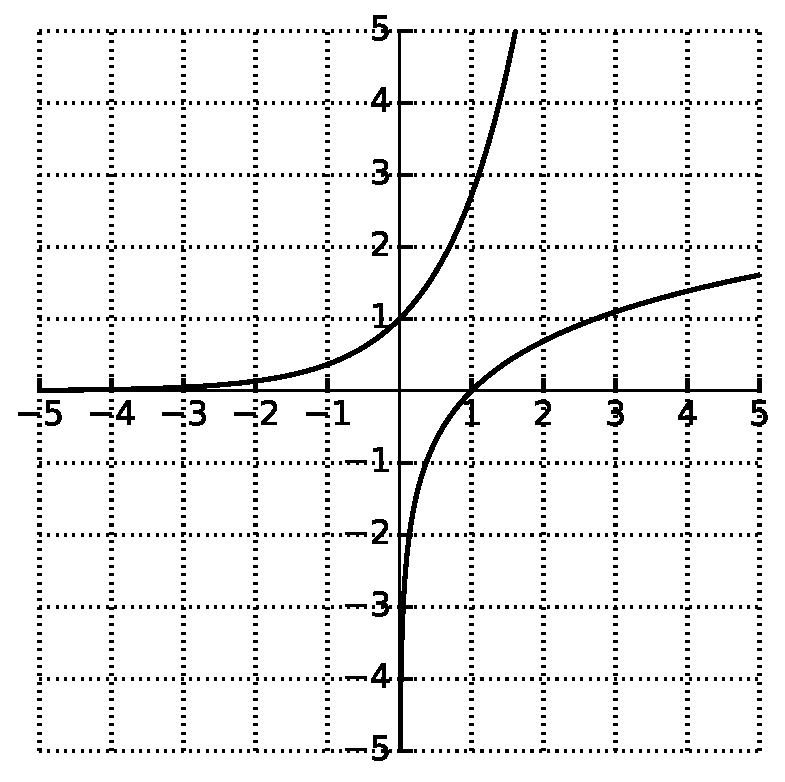
\includegraphics[width=0.5\textwidth]{img/exp.pdf}
%\caption{$y=\exp(x)$ und $y=\ln(x)$}
%\end{figure}

\subsection{Winkelfunktionen}\index{Winkelfunktion}
\begin{definition}[Winkelfunktionen]\mbox{}\newline
\emdef{Sinus}\index{Sinus}: $\C\to\C$,
\begin{equation}
\sin(x) := \sum_{k=0}^\infty \frac{x^{2k+1}}{(2k+1)!}
= x+\frac{x^3}{3!}+\frac{x^5}{5!}+\ldots
\end{equation}
\emdef{Kosinus}\index{Kosinus}\index{Cosinus}: $\C\to\C$,
\begin{equation}
\cos(x) := \sum_{k=0}^\infty \frac{x^{2k}}{(2k)!}
= 1+\frac{x^2}{2!}+\frac{x^4}{4!}+\ldots
\end{equation}
\emdef{Tangens}\index{Tangens}: $\C\setminus\{k\pi+\pi/2\mid k\in\Z\}\to\C$,
\begin{equation}
\tan(x) := \frac{\sin(x)}{\cos(x)}.
\end{equation}
\emdef{Kotangens}\index{Kotangens}: $\C\setminus\{k\pi\mid k\in\Z\}\to\C$,
\begin{equation}
\cot(x) := \frac{\cos(x)}{\sin(x)}.
\end{equation}
\emdef{Sekans}\index{Sekans}: $\C\setminus\{k\pi+\pi/2\mid k\in\Z\}\to\C$,
\begin{equation}
\sec(x) := \frac{1}{\cos(x)}.
\end{equation}
\emdef{Kosekans}\index{Kosekans}: $\C\setminus\{k\pi\mid k\in\Z\}\to\C$,
\begin{equation}
\csc(x) := \frac{1}{\sin(x)}.
\end{equation}
\end{definition}
\noindent
Darstellung durch die Exponentialfunktion:\\
Für $x\in\C$ gilt:
\begin{align}
\cos x &= \real(\ee^{\ui x}) = \frac{\ee^{\ui x}+\ee^{-\ui x}}{2},\\
\sin x &= \imag(\ee^{\ui x}) = \frac{\ee^{\ui x}-\ee^{-\ui x}}{2\ui}.
\end{align}
Die Funktionen $\sin, \cos$ sind holomorph auf ganz $\C$.
Die Ableitungen sind
\begin{align}
\sin' x &= \cos x,\\
\cos' x &= -\sin x.
\end{align}

\subsubsection{Symmetrie und Periodizität}
Für $x\in\C$ gilt:
\begin{align}
\sin(-x) &= -\sin x,\enspace(\text{Punktsymmetrie})\\
\cos(-x) &= \cos x,\quad\;(\text{Achsensymmetrie})\\
\sin(x+2\pi) &= \sin x,\\
\cos(x+2\pi) &= \cos x,\\
\sin(x+\pi)  &=-\sin x,\\
\cos(x+\pi)  &=-\cos x,\\
\sin\Big(x+\frac{\pi}{2}\Big) &= \cos x = -\sin\Big(x-\frac{\pi}{2}\Big),\\
\cos\Big(x+\frac{\pi}{2}\Big) &= -\sin x = -\cos\Big(x-\frac{\pi}{2}\Big).
\end{align}

\subsubsection{Additionstheoreme}
\index{Additionstheoreme}

Für $x,y\in\C$ gilt:
\begin{align}
\sin(x+y) &= \sin x\cos y+\cos x\sin y,\\
\sin(x-y) &= \sin x\cos y-\cos x\sin y,\\
\cos(x+y) &= \cos x\cos y-\sin x\sin y,\\
\cos(x-y) &= \cos x\cos y+\sin x\sin y.
\end{align}

\subsubsection{Trigonometrischer Pythagoras}
Für $x\in\C$ gilt:
\begin{equation}
\sin^2 x+\cos^2 x=1.
\end{equation}

\subsubsection{Produkte}
Für $x,y\in\C$ gilt:
\begin{align}
2\sin x\sin y &= \cos(x-y)-\cos(x+y),\\
2\cos x\cos y &= \cos(x-y)+\cos(x+y),\\
2\sin x\cos y &= \sin(x-y)+\sin(x+y).
\end{align}

\subsubsection{Summen und Differenzen}
Für $x,y\in\C$ gilt:
\begin{align}
\sin x+\sin y &= 2\sin\frac{x+y}{2}\cos\frac{x-y}{2},\\
\sin x-\sin y &= 2\cos\frac{x+y}{2}\sin\frac{x-y}{2},\\
\cos x+\cos y &= 2\cos\frac{x+y}{2}\cos\frac{x-y}{2},\\
\cos x-\cos y &= 2\sin\frac{x+y}{2}\sin\frac{y-x}{2}.
\end{align}

\subsubsection{Winkelvielfache}
Für $x\in\C$ gilt:
\begin{align}
\sin(2x) &= 2\sin x\cos x,\\
\cos(2x) &= \cos^2 x-\sin^2 x,\\
\sin(3x) &= 3\sin x-4\sin^3 x,\\
\cos(3x) &= 4\cos^3 x-3\cos x.
\end{align}
Zusätzlich gilt:
\begin{align}
\cos(2x) &= 1-2\sin^2 x = 2\cos^2 x-1.
\end{align}
Rekursionsformeln für $x,n\in\C$:
\begin{align}
\hspace{-1em}\cos(nx) &= 2\cos x \cos((n{-}1)x) - \cos((n{-}2)x),\\
\hspace{-1em}\sin(nx) &= 2\cos x \sin((n{-}2)x) - \sin((n{-}2)x).
\end{align}

\begin{figure}[h]
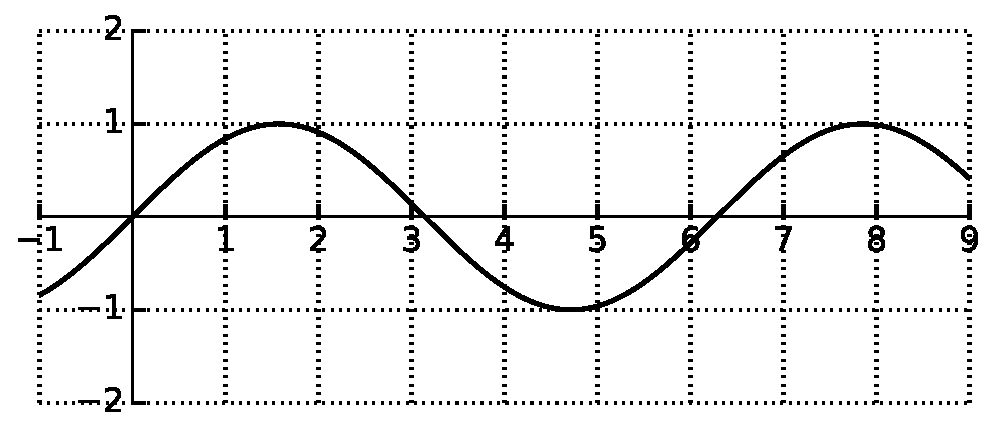
\includegraphics[width=0.5\textwidth]{img/sin.pdf}
\caption{$y=\sin(x)$}
\end{figure}

\begin{figure}[h]
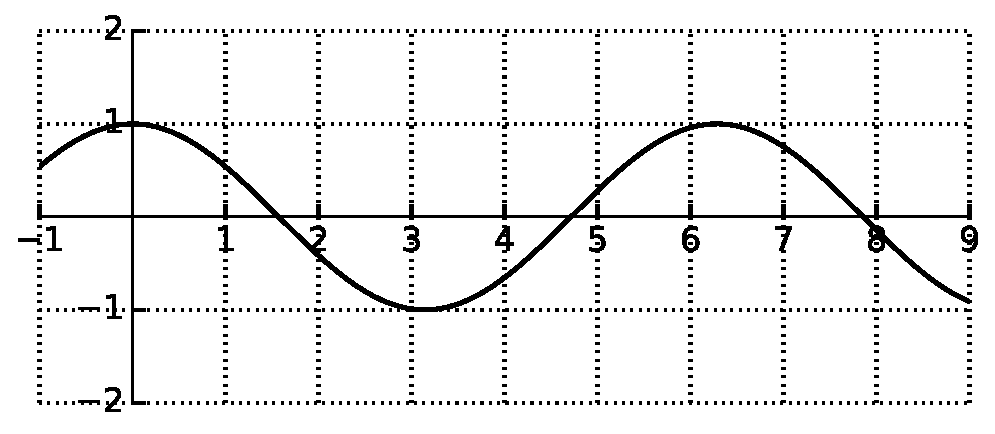
\includegraphics[width=0.5\textwidth]{img/cos.pdf}
\caption{$y=\cos(x)$}
\end{figure}

\begin{figure}[h]
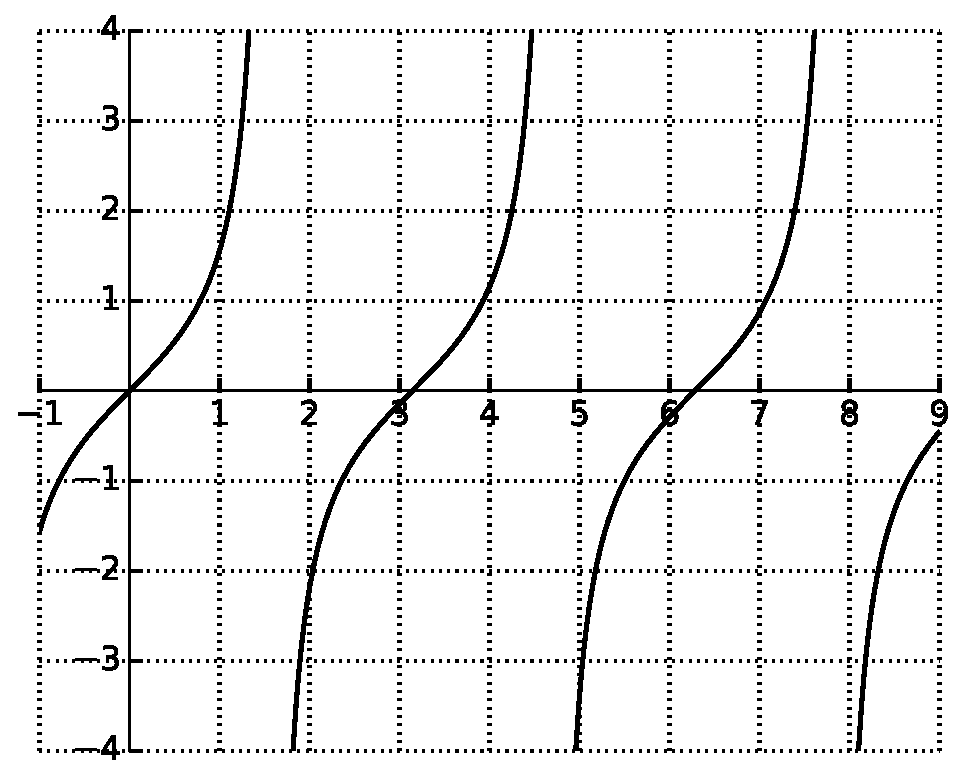
\includegraphics[width=0.5\textwidth]{img/tan.pdf}
\caption{$y=\tan(x)$}
\end{figure}

\begin{figure}[h]
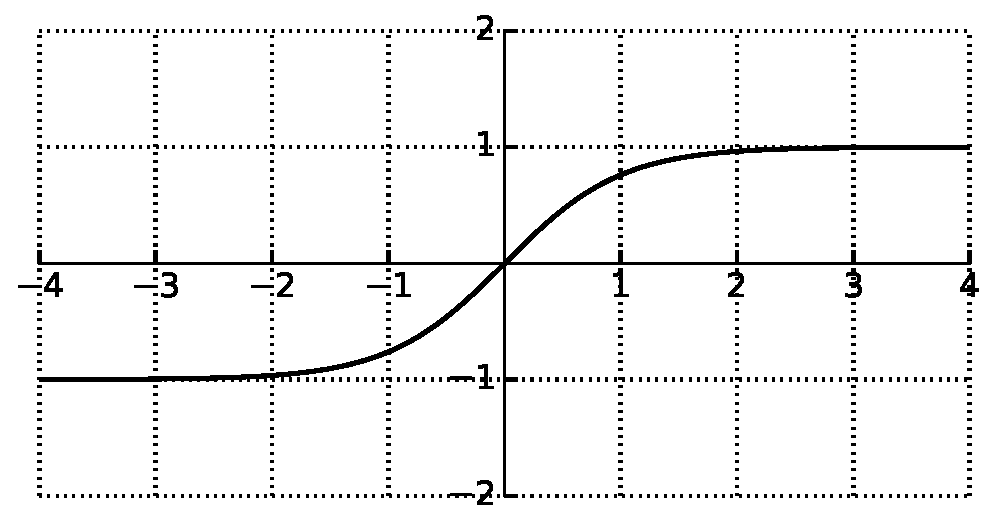
\includegraphics[width=0.5\textwidth]{img/tanh.pdf}
\caption{$y=\tanh(x)$}
\end{figure}

\newpage
\section{Zahlentheoretische Funktionen}
\subsection{Eulersche Phi-Funktion}

\begin{definition}[Eulersche Phi-Funktion]\mbox{}\newline
Für $n\in\N$:
\begin{equation}
\varphi(n) := |\{a{\in}\N\mid 1{\le}a{\le}n\wedge\operatorname{ggT}(a,n){=}1\}|.
\end{equation}
\end{definition}

\noindent
Für zwei teilerfremde Zahlen $m,n$ gilt:
\begin{equation}
\varphi(mn) = \varphi(m)\,\varphi(n).
\end{equation}
Für jede Primzahlpotenz $p^k$ mit $k\in\Z$ und $k\ge 1$ gilt:
\begin{equation}
\varphi(p^k) = p^k-p^{k-1}.
\end{equation}
Für eine Zahl $n$ mit der Primfaktorzerlegung
\begin{equation}
n=\prod_{p|n} p^{k_p}
\end{equation}
gilt:
\begin{equation}
\varphi(n) = \prod_{p|n} (p^{k_p}-p^{k_p-1})
= n\prod_{p|n} \Big(1-\frac{1}{p}\Big).
\end{equation}

\subsection{Carmichael-Funktion}
\begin{definition}[Carmichael-Funktion]\mbox{}\newline
Für $n\in\N$:
\begin{equation}
\begin{split}
\lambda(n) &:= \min\{m\mid \forall a(\operatorname{ggT}(a,n)=1\\
&\implies a^m\equiv 1\mod n)\}.
\end{split}
\end{equation}
\end{definition}
